% SPL 在线补充材料（2026-11-17）。表格由 scripts/spl_supplement.py 从原始逐样本 CSV / 冻结账本一次舍入生成（paper/spl/supp/*.tex）。
% 编译：python scripts/spl_supplement.py && cd paper/spl && latexmk -pdf supplement.tex
\documentclass[10pt,letterpaper]{article}
\usepackage[letterpaper,margin=0.8in]{geometry}
\usepackage[T1]{fontenc}
\usepackage{mathptmx}
\renewcommand{\ttdefault}{pcr}
\usepackage{amsmath,booktabs,longtable,graphicx,xcolor,array,float}
\usepackage[hyphens]{url}
\renewcommand{\UrlBreaks}{\do\/\do\_\do\,\do\-}
\emergencystretch=2em
\usepackage[hidelinks]{hyperref}
\renewcommand{\thesection}{S\arabic{section}}
\renewcommand{\thetable}{S\arabic{table}}
\renewcommand{\thefigure}{S\arabic{figure}}
\setlength{\parindent}{0pt}\setlength{\parskip}{4pt}
\title{Supplementary Material for ``What Relaxing Convexity Buys and Costs in Neural Fusion of Distortionless Beamformers''}
\author{Lingnan Liu\\\normalsize College of Electronic Engineering, Ocean University of China, Qingdao 266404, China}
\date{}
\begin{document}
\sloppy
\maketitle
\small
Code, per-utterance results, analysis ledgers, and this document are available at\newline\mbox{\url{https://github.com/Knight11239/cr-beamfusion-spl}}.

All tables below are generated by \path|scripts/spl_supplement.py| from the saved per-utterance results and the frozen analysis ledger; every displayed value is rounded once from the unrounded mean or paired difference. A$=$G2-Affine-mm or Affine-mm, B$=$BeamFusion-mm, C$=$convex model with the matched output layer, R$=$real affine, F$=$unconstrained fusion. Unless stated otherwise, the metric is $\Delta$SI-SDR with respect to $x_{\mathrm{dp}}$ in dB. Sections~\ref{sec:floors} and~\ref{sec:bands} are post hoc and exploratory.

\section{Pre-Registered Comparisons: Complete Tables}
\label{sec:primary}
The analysis plan (\path|research/analysis_plan_controls.md|, v1.1) was frozen before the control models were trained; the earlier A and B results were already known. Table~\ref{tab:primary} lists all 56 primary tests (50 two-sided paired Wilcoxon tests and six paired-mean TOST equivalence tests for C1 with margin $\pm0.5$\,dB), with means of per-utterance paired differences ($n=600$ per cell), per-utterance 95\% intervals ($90\%$ for TOST), and $p$ values after the global Holm correction. H8: 8-microphone comparisons C1--C5; HF: pre-specified diagnostics of F against A (nominal response deviation, frozen target-direct distortion, extra degradation under mismatch); HG2: G2 simulation comparisons G1 (A$-$B) and G2 (B minus the same convex model trained without augmentation). C2 (R$-$C) and C3 (A$-$R), summarized in one sentence in the letter, appear here in full. Table~\ref{tab:mird} gives the separate six-test MIRD family (M1--M3 $\times$ S1/S2), evaluated on the six $T_{60}$--subarray condition means; with six conditions the smallest attainable two-sided signed-rank $p$ is 0.03125, so no Holm-corrected $p<0.05$ is attainable in this family.
{\scriptsize\begin{longtable}{@{}llllrrrr@{}}
\caption{All 56 primary tests (frozen plan; global Holm correction).}\label{tab:primary}\\
\toprule
Comp. & Family & Scen. & $\kappa$ & Kind & Mean diff. & 95\% CI & Holm-56 $p$ \\
\midrule\endhead
C1 & H8 & S1 & 0 & diff., \texttt{d\_si\_sdr\_dp} & +2.166 & [2.11, 2.22] & $3.3\times10^{-98}$ \\
C1 & H8 & S1 & 1 & diff., \texttt{d\_si\_sdr\_dp} & +2.127 & [2.05, 2.20] & $3.3\times10^{-98}$ \\
C1 & H8 & S1 & 2 & diff., \texttt{d\_si\_sdr\_dp} & +1.542 & [1.41, 1.67] & $2.8\times10^{-71}$ \\
C1 & H8 & S2 & 0 & diff., \texttt{d\_si\_sdr\_dp} & +2.027 & [1.97, 2.08] & $3.3\times10^{-98}$ \\
C1 & H8 & S2 & 1 & diff., \texttt{d\_si\_sdr\_dp} & +1.900 & [1.83, 1.97] & $3.3\times10^{-98}$ \\
C1 & H8 & S2 & 2 & diff., \texttt{d\_si\_sdr\_dp} & +1.279 & [1.16, 1.40] & $7.3\times10^{-62}$ \\
C2 & H8 & S1 & 0 & diff., \texttt{d\_si\_sdr\_dp} & +0.693 & [0.64, 0.75] & $1.4\times10^{-74}$ \\
C2 & H8 & S1 & 1 & diff., \texttt{d\_si\_sdr\_dp} & +0.113 & [0.04, 0.18] & $2.5\times10^{-5}$ \\
C2 & H8 & S1 & 2 & diff., \texttt{d\_si\_sdr\_dp} & $-$1.299 & [$-$1.60, $-$1.00] & $3.6\times10^{-23}$ \\
C2 & H8 & S2 & 0 & diff., \texttt{d\_si\_sdr\_dp} & +0.748 & [0.70, 0.80] & $9.2\times10^{-84}$ \\
C2 & H8 & S2 & 1 & diff., \texttt{d\_si\_sdr\_dp} & +0.134 & [0.06, 0.21] & $7.0\times10^{-6}$ \\
C2 & H8 & S2 & 2 & diff., \texttt{d\_si\_sdr\_dp} & $-$1.474 & [$-$1.80, $-$1.15] & $8.2\times10^{-24}$ \\
C3 & H8 & S1 & 0 & diff., \texttt{d\_si\_sdr\_dp} & +1.473 & [1.42, 1.53] & $3.3\times10^{-98}$ \\
C3 & H8 & S1 & 1 & diff., \texttt{d\_si\_sdr\_dp} & +2.015 & [1.93, 2.10] & $3.3\times10^{-98}$ \\
C3 & H8 & S1 & 2 & diff., \texttt{d\_si\_sdr\_dp} & +2.840 & [2.58, 3.10] & $2.0\times10^{-97}$ \\
C3 & H8 & S2 & 0 & diff., \texttt{d\_si\_sdr\_dp} & +1.279 & [1.23, 1.33] & $3.3\times10^{-98}$ \\
C3 & H8 & S2 & 1 & diff., \texttt{d\_si\_sdr\_dp} & +1.766 & [1.69, 1.84] & $3.3\times10^{-98}$ \\
C3 & H8 & S2 & 2 & diff., \texttt{d\_si\_sdr\_dp} & +2.753 & [2.48, 3.03] & $1.8\times10^{-96}$ \\
C4 & H8 & S1 & 0 & diff., \texttt{d\_si\_sdr\_dp} & $-$0.088 & [$-$0.09, $-$0.08] & $1.7\times10^{-87}$ \\
C4 & H8 & S1 & 1 & diff., \texttt{d\_si\_sdr\_dp} & $-$0.107 & [$-$0.12, $-$0.10] & $4.2\times10^{-82}$ \\
C4 & H8 & S1 & 2 & diff., \texttt{d\_si\_sdr\_dp} & $-$0.110 & [$-$0.12, $-$0.10] & $7.8\times10^{-68}$ \\
C4 & H8 & S2 & 0 & diff., \texttt{d\_si\_sdr\_dp} & $-$0.092 & [$-$0.10, $-$0.09] & $2.1\times10^{-89}$ \\
C4 & H8 & S2 & 1 & diff., \texttt{d\_si\_sdr\_dp} & $-$0.108 & [$-$0.12, $-$0.10] & $1.6\times10^{-88}$ \\
C4 & H8 & S2 & 2 & diff., \texttt{d\_si\_sdr\_dp} & $-$0.108 & [$-$0.12, $-$0.10] & $4.4\times10^{-66}$ \\
C5 & H8 & S1 & 0 & diff., \texttt{d\_si\_sdr\_dp} & +1.900 & [1.84, 1.96] & $3.3\times10^{-98}$ \\
C5 & H8 & S1 & 1 & diff., \texttt{d\_si\_sdr\_dp} & +2.079 & [2.01, 2.15] & $6.0\times10^{-98}$ \\
C5 & H8 & S1 & 2 & diff., \texttt{d\_si\_sdr\_dp} & +2.697 & [2.59, 2.81] & $4.1\times10^{-98}$ \\
C5 & H8 & S2 & 0 & diff., \texttt{d\_si\_sdr\_dp} & +1.965 & [1.90, 2.02] & $3.3\times10^{-98}$ \\
C5 & H8 & S2 & 1 & diff., \texttt{d\_si\_sdr\_dp} & +2.171 & [2.10, 2.24] & $3.3\times10^{-98}$ \\
C5 & H8 & S2 & 2 & diff., \texttt{d\_si\_sdr\_dp} & +2.773 & [2.66, 2.88] & $3.3\times10^{-98}$ \\
C1 & H8 & S1 & 0 & TOST, \texttt{d\_si\_sdr\_dp} & +2.166 & [2.12, 2.21]$^{90}$ & 1.000 \\
F\_D & HF & S1 & 0 & diff., \texttt{nominal\_D\_p95} & +0.952 & [0.95, 0.95] & $3.3\times10^{-98}$ \\
F\_TD & HF & S1 & 0 & diff., \texttt{target\_direct\_sdr\_out} & $-$12.258 & [$-$12.53, $-$11.98] & $3.3\times10^{-98}$ \\
C1 & H8 & S1 & 1 & TOST, \texttt{d\_si\_sdr\_dp} & +2.127 & [2.06, 2.19]$^{90}$ & 1.000 \\
F\_D & HF & S1 & 1 & diff., \texttt{nominal\_D\_p95} & +0.953 & [0.95, 0.96] & $3.3\times10^{-98}$ \\
F\_TD & HF & S1 & 1 & diff., \texttt{target\_direct\_sdr\_out} & $-$6.825 & [$-$7.18, $-$6.47] & $7.6\times10^{-96}$ \\
F\_R & HF & S1 & 1 & degr., \texttt{d\_si\_sdr\_dp} & +0.179 & [0.14, 0.22] & $8.7\times10^{-19}$ \\
C1 & H8 & S1 & 2 & TOST, \texttt{d\_si\_sdr\_dp} & +1.542 & [1.43, 1.65]$^{90}$ & 1.000 \\
F\_D & HF & S1 & 2 & diff., \texttt{nominal\_D\_p95} & +0.955 & [0.95, 0.96] & $3.3\times10^{-98}$ \\
F\_TD & HF & S1 & 2 & diff., \texttt{target\_direct\_sdr\_out} & $-$3.069 & [$-$3.35, $-$2.78] & $7.6\times10^{-64}$ \\
F\_R & HF & S1 & 2 & degr., \texttt{d\_si\_sdr\_dp} & +0.797 & [0.70, 0.90] & $1.9\times10^{-51}$ \\
C1 & H8 & S2 & 0 & TOST, \texttt{d\_si\_sdr\_dp} & +2.027 & [1.98, 2.07]$^{90}$ & 1.000 \\
F\_D & HF & S2 & 0 & diff., \texttt{nominal\_D\_p95} & +0.956 & [0.95, 0.96] & $3.3\times10^{-98}$ \\
F\_TD & HF & S2 & 0 & diff., \texttt{target\_direct\_sdr\_out} & $-$12.378 & [$-$12.66, $-$12.09] & $3.3\times10^{-98}$ \\
C1 & H8 & S2 & 1 & TOST, \texttt{d\_si\_sdr\_dp} & +1.900 & [1.84, 1.96]$^{90}$ & 1.000 \\
F\_D & HF & S2 & 1 & diff., \texttt{nominal\_D\_p95} & +0.957 & [0.96, 0.96] & $3.3\times10^{-98}$ \\
F\_TD & HF & S2 & 1 & diff., \texttt{target\_direct\_sdr\_out} & $-$7.069 & [$-$7.41, $-$6.73] & $1.3\times10^{-96}$ \\
F\_R & HF & S2 & 1 & degr., \texttt{d\_si\_sdr\_dp} & +0.206 & [0.16, 0.25] & $3.8\times10^{-21}$ \\
C1 & H8 & S2 & 2 & TOST, \texttt{d\_si\_sdr\_dp} & +1.279 & [1.18, 1.38]$^{90}$ & 1.000 \\
F\_D & HF & S2 & 2 & diff., \texttt{nominal\_D\_p95} & +0.958 & [0.96, 0.96] & $3.3\times10^{-98}$ \\
F\_TD & HF & S2 & 2 & diff., \texttt{target\_direct\_sdr\_out} & $-$3.341 & [$-$3.62, $-$3.07] & $9.8\times10^{-73}$ \\
F\_R & HF & S2 & 2 & degr., \texttt{d\_si\_sdr\_dp} & +0.808 & [0.71, 0.91] & $9.1\times10^{-51}$ \\
G1 & HG2 & S1 & 0 & diff., \texttt{d\_si\_sdr\_dp} & +0.924 & [0.88, 0.97] & $1.5\times10^{-95}$ \\
G1 & HG2 & S2 & 0 & diff., \texttt{d\_si\_sdr\_dp} & +0.824 & [0.78, 0.87] & $8.0\times10^{-93}$ \\
G2 & HG2 & S1 & 0 & diff., \texttt{d\_si\_sdr\_dp} & +0.011 & [0.01, 0.02] & $7.4\times10^{-5}$ \\
G2 & HG2 & S2 & 0 & diff., \texttt{d\_si\_sdr\_dp} & +0.008 & [0.00, 0.01] & 0.059 \\
\bottomrule
\end{longtable}
}
\begin{table}[H]\centering\caption{MIRD family (seed 0): M1 $=$ A$-$B, M2 $=$ learned-floor affine model $-$ B, M3 $=$ B minus its non-augmented counterpart.}\label{tab:mird}
{\footnotesize\begin{tabular}{@{}llrrrr@{}}
\toprule
Comp. & Scen. & Mean (6 cond.) & $t_5$ 95\% CI & Cond.\ $>0$ & Holm-6 $p$ \\
\midrule
M1 & S1 & $-$0.62 & [$-$1.15, $-$0.10] & 0 & 0.188 \\
M1 & S2 & $-$0.57 & [$-$1.03, $-$0.11] & 0 & 0.188 \\
M2 & S1 & $-$0.51 & [$-$1.44, 0.42] & 2 & 0.312 \\
M2 & S2 & $-$0.48 & [$-$1.34, 0.37] & 2 & 0.312 \\
M3 & S1 & +0.11 & [0.07, 0.15] & 6 & 0.188 \\
M3 & S2 & +0.10 & [0.05, 0.15] & 6 & 0.188 \\
\bottomrule
\end{tabular}
}\end{table}

\section{Windowed Oracle Fits}
\label{sec:oracle}
For each frequency and non-overlapping window of $L$ frames, one weight vector is fitted over the convex, real-affine, or complex-affine set by minimizing the STFT-domain squared error to the reference with relative diagonal loading $\rho=10^{-9}$ (8-microphone, $\kappa=0$, a fixed subset of $n=100$ utterances per scenario). ``In-window'' applies the fit to the same window; ``next-window'' applies window $k$'s weights to window $k+1$. Values are absolute waveform SI-SDR (dB), not $\Delta$SI-SDR. These fits probe the capacity of the feasible sets under a regularized MSE; they are not SI-SDR upper bounds and do not evaluate the trained networks (source: \path|results/oracle/|).
\begin{table}[H]\centering\caption{Windowed oracle fits (absolute SI-SDR, dB).}{\footnotesize\begin{tabular}{@{}llllrrr@{}}
\toprule
Scen. & Target & Part & $L$ & Convex & Real affine & Complex affine \\
\midrule
S1 & $x_{\mathrm{dp}}$ & in-window & 8 & 0.04 & 5.36 & 9.40 \\
S1 & $x_{\mathrm{dp}}$ & in-window & 32 & $-$0.35 & 3.71 & 5.40 \\
S1 & $x_{\mathrm{dp}}$ & in-window & 125 & $-$0.52 & 3.08 & 4.17 \\
S1 & $x_{\mathrm{dp}}$ & out-of-window & 8 & $-$1.08 & 0.60 & 0.21 \\
S1 & $x_{\mathrm{dp}}$ & out-of-window & 32 & $-$1.30 & 0.91 & 0.92 \\
S1 & $x_{\mathrm{dp}}$ & out-of-window & 125 & $-$1.85 & 0.12 & 0.27 \\
S1 & $x_{\mathrm{ref}}$ & in-window & 8 & 6.91 & 10.21 & 14.05 \\
S1 & $x_{\mathrm{ref}}$ & in-window & 32 & 5.77 & 7.50 & 8.94 \\
S1 & $x_{\mathrm{ref}}$ & in-window & 125 & 5.10 & 6.30 & 7.21 \\
S1 & $x_{\mathrm{ref}}$ & out-of-window & 8 & 4.31 & 4.36 & 4.00 \\
S1 & $x_{\mathrm{ref}}$ & out-of-window & 32 & 3.37 & 3.45 & 3.49 \\
S1 & $x_{\mathrm{ref}}$ & out-of-window & 125 & 3.28 & 3.58 & 3.74 \\
S2 & $x_{\mathrm{dp}}$ & in-window & 8 & $-$0.52 & 5.00 & 8.91 \\
S2 & $x_{\mathrm{dp}}$ & in-window & 32 & $-$0.93 & 3.32 & 4.87 \\
S2 & $x_{\mathrm{dp}}$ & in-window & 125 & $-$1.10 & 2.71 & 3.66 \\
S2 & $x_{\mathrm{dp}}$ & out-of-window & 8 & $-$1.61 & 0.51 & $-$0.01 \\
S2 & $x_{\mathrm{dp}}$ & out-of-window & 32 & $-$1.79 & 0.75 & 0.67 \\
S2 & $x_{\mathrm{dp}}$ & out-of-window & 125 & $-$2.27 & $-$0.04 & 0.10 \\
S2 & $x_{\mathrm{ref}}$ & in-window & 8 & 5.55 & 9.21 & 13.00 \\
S2 & $x_{\mathrm{ref}}$ & in-window & 32 & 4.44 & 6.40 & 7.79 \\
S2 & $x_{\mathrm{ref}}$ & in-window & 125 & 3.77 & 5.11 & 5.95 \\
S2 & $x_{\mathrm{ref}}$ & out-of-window & 8 & 3.07 & 3.20 & 2.72 \\
S2 & $x_{\mathrm{ref}}$ & out-of-window & 32 & 2.04 & 2.15 & 2.16 \\
S2 & $x_{\mathrm{ref}}$ & out-of-window & 125 & 2.29 & 2.64 & 2.84 \\
\bottomrule
\end{tabular}
}\end{table}
\begin{figure}[H]\centering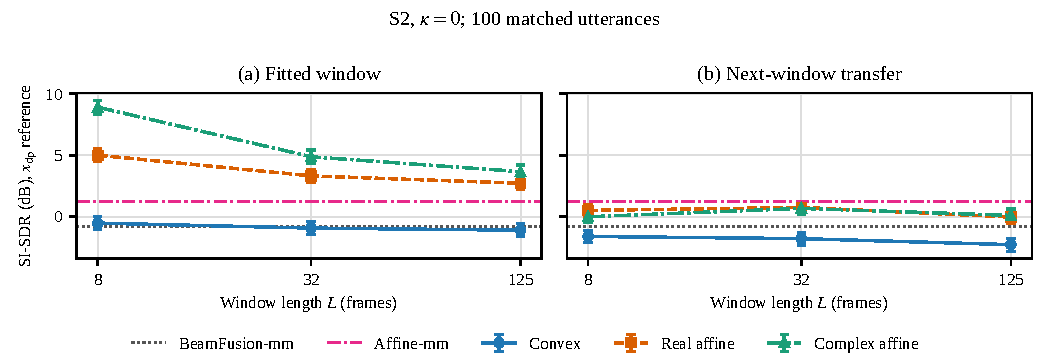
\includegraphics[width=0.9\textwidth]{../figures/supplement/fig_oracle_s2_x_dp}\caption{Windowed oracle fits, S2, $x_{\mathrm{dp}}$; horizontal lines: causal Affine-mm and BeamFusion-mm on the same utterances.}\end{figure}

\section{Baseline Tuning}
\label{sec:tuning}
Hyperparameters were chosen on validation data only (500 mixtures), by mean $\Delta$SI-SDR ($x_{\mathrm{dp}}$). ``Nominal'' denotes the validation set without mismatch; ``mismatched'' denotes the same set with fixed per-utterance gain and phase errors ($\kappa\sim\mathcal U[0,1]$), as used for ``-mm'' training. The letter reports the mask-based MVDR and DMA-GSC-MPDR tuned on the mismatched set and ACC tuned on the nominal set. For ACC on G2, the grid was extended downwards until the selected step size was interior. DMA-GSC-MPDR grids: forgetting factor $\lambda\in\{0.9,\dots,0.9995,1\}$ (nine values; $\lambda=1$ is the running average from the start of the utterance) and relative loading $\delta_{\mathrm{load}}\in\{3\times10^{-7},10^{-6},\dots,10^{-2}\}$; selection records: \path|results/baselines2/mpdr_select*.json|.
\begin{table}[H]\centering\caption{Validation scores of the tuning grids and selected values.}{\scriptsize\begin{tabular}{@{}p{3.3cm}p{10.2cm}p{2.6cm}@{}}
\toprule
Baseline (array; validation set) & Candidates (mean $\Delta$SI-SDR, dB) & Selected \\
\midrule
ACC $\mu$ ($M{=}8$; nominal) & 0.001: 4.92, 0.003: 5.21, 0.01: 5.47, 0.03: 5.57, 0.1: 5.54, 0.3: 5.39 & 0.03 \\
Mask-MVDR loading ($M{=}8$; mismatched) & 1e-06: $-$3.99, 1e-05: $-$3.22, 0.0001: $-$0.08, 0.001: 4.98, 0.01: 6.52, 0.1: 4.14 & 0.01 \\
ACC $\mu$ (G2; nominal) & 0.0: 1.65, 3e-05: 2.21, 0.0001: 3.33, 0.0003: 4.24, 0.001: 4.32, 0.003: 1.54, 0.01: $-$2.83, 0.03: $-$3.58, 0.1: $-$2.05, 0.3: 0.99 & 0.001 \\
DMA-GSC-MPDR ($M{=}8$; nominal) & top 3: $\lambda$=1,$\delta_{\mathrm{load}}$=1e-06: 6.03; $\lambda$=1,$\delta_{\mathrm{load}}$=3e-07: 6.01; $\lambda$=0.9995,$\delta_{\mathrm{load}}$=1e-06: 6.00 & $\lambda$=1,$\delta_{\mathrm{load}}$=1e-06 \\
DMA-GSC-MPDR ($M{=}8$; mismatched) & top 3: $\lambda$=1,$\delta_{\mathrm{load}}$=0.0001: 5.04; $\lambda$=0.9995,$\delta_{\mathrm{load}}$=0.0001: 5.02; $\lambda$=1,$\delta_{\mathrm{load}}$=0.001: 5.02 & $\lambda$=1,$\delta_{\mathrm{load}}$=0.0001 \\
DMA-GSC-MPDR (G2; nominal) & top 3: $\lambda$=1,$\delta_{\mathrm{load}}$=1e-05: 5.93; $\lambda$=1,$\delta_{\mathrm{load}}$=1e-06: 5.91; $\lambda$=0.9995,$\delta_{\mathrm{load}}$=1e-05: 5.90 & $\lambda$=1,$\delta_{\mathrm{load}}$=1e-05 \\
DMA-GSC-MPDR (G2; mismatched) & top 3: $\lambda$=1,$\delta_{\mathrm{load}}$=0.001: 4.98; $\lambda$=0.9995,$\delta_{\mathrm{load}}$=0.001: 4.97; $\lambda$=0.999,$\delta_{\mathrm{load}}$=0.001: 4.95 & $\lambda$=1,$\delta_{\mathrm{load}}$=0.001 \\
\bottomrule
\end{tabular}
}\end{table}

\section{Training-Target Comparison (Not Pre-Registered)}
\label{sec:xref}
This comparison predates the analysis plan and is not part of it. Affine and convex (original BeamFusion head) models were both trained on $x_{\mathrm{ref}}$ (direct path plus 50\,ms of early reflections) without mismatch augmentation, seed 0 (sources: \path|results/kaggle/b5-eval-s{1,2}|; checkpoints \path|results/checkpoints/stage4-train-b5/affine_xref_best.pt| (Affine-xref) and \path|results/checkpoints/stage3-train/beamfusion_best.pt| (BeamFusion-xref)). Table~\ref{tab:xref} gives Affine-xref $-$ BeamFusion-xref on both references with per-utterance 95\% intervals.
\begin{table}[H]\centering\caption{Affine-xref $-$ BeamFusion-xref (dB, $n=600$ per cell).}\label{tab:xref}{\footnotesize\begin{tabular}{@{}llrrrr@{}}
\toprule
Scen. & $\kappa$ & $x_{\mathrm{ref}}$: diff. & 95\% CI & $x_{\mathrm{dp}}$: diff. & 95\% CI \\
\midrule
S1 & 0 & +1.59 & [1.52, 1.65] & $-$0.30 & [$-$0.33, $-$0.27] \\
S1 & 1 & +1.63 & [1.57, 1.70] & $-$0.21 & [$-$0.25, $-$0.18] \\
S1 & 2 & +1.42 & [1.26, 1.58] & $-$0.30 & [$-$0.40, $-$0.19] \\
S2 & 0 & +1.53 & [1.48, 1.58] & $-$0.21 & [$-$0.24, $-$0.18] \\
S2 & 1 & +1.53 & [1.46, 1.60] & $-$0.14 & [$-$0.17, $-$0.11] \\
S2 & 2 & +1.30 & [1.19, 1.42] & $-$0.22 & [$-$0.30, $-$0.15] \\
\bottomrule
\end{tabular}
}\end{table}

\section{Exploratory: Equal Inference-Time WNG Floors}
\label{sec:floors}
These analyses were proposed after the MIRD results had been seen (plans: \path|results/explore/PLAN.md|, \path|PLAN2.md|). The scaled projection of the letter is applied at inference to frozen models; convex weights map to $u_p=\alpha_p$ ($p\ge1$) and remain in the simplex. For seed 0 the full grid was evaluated; for seeds 1 and 2 only the unprojected models and $-5$\,dB. A rule fixed before these results (seed 0; highest mean validation score over the five floors, unprojected models excluded) selects $-15$\,dB for both models. The value $-5$\,dB was examined because it was the highest on MIRD for seed 0; it is not a selection.
\begin{table}[H]\centering\caption{Equal floors: validation (mismatched simulation, 500 mixtures) and MIRD ($\Delta$SI-SDR, six-condition means; in brackets, conditions with A$>$B out of 6).}{\scriptsize\begin{tabular}{@{}llrrrrrr@{}}
\toprule
Seed & Floor & Val.\ A & Val.\ B & MIRD A (S1/S2) & MIRD B (S1/S2) & A$-$B S1 & A$-$B S2 \\
\midrule
0 & none & 7.14 & 6.19 & 4.04/3.43 & 4.66/4.00 & $-$0.62 (0) & $-$0.57 (0) \\
0 & $-$15\,dB & 6.88 & 6.11 & 4.04/3.44 & 4.66/4.00 & $-$0.62 (0) & $-$0.56 (0) \\
0 & $-$10\,dB & 6.35 & 5.82 & 4.14/3.54 & 4.71/4.05 & $-$0.56 (0) & $-$0.50 (1) \\
0 & $-$5\,dB & 5.21 & 5.05 & 5.33/4.63 & 5.33/4.62 & +0.00 (2) & +0.01 (3) \\
0 & 0\,dB & 3.68 & 3.73 & 4.47/3.80 & 4.48/3.82 & $-$0.01 (3) & $-$0.01 (2) \\
0 & 3\,dB & 2.62 & 2.70 & 3.14/2.66 & 3.19/2.70 & $-$0.05 (1) & $-$0.04 (2) \\
1 & none & 7.40 & 6.08 & 3.44/2.87 & 4.63/3.98 & $-$1.19 (0) & $-$1.12 (0) \\
1 & $-$5\,dB & 5.29 & 5.00 & 5.00/4.33 & 5.32/4.62 & $-$0.33 (0) & $-$0.29 (0) \\
2 & none & 7.02 & 6.05 & 3.34/2.85 & 4.53/3.89 & $-$1.18 (0) & $-$1.04 (0) \\
2 & $-$5\,dB & 5.06 & 4.98 & 5.01/4.38 & 5.33/4.64 & $-$0.32 (0) & $-$0.26 (0) \\
\bottomrule
\end{tabular}
}\end{table}
\begin{table}[H]\centering\caption{MIRD, A$-$B on secondary metrics without floors and with equal $-5$\,dB floors (six-condition means).}{\scriptsize\begin{tabular}{@{}llrrrr@{}}
\toprule
Seed & Floor & $x_{\mathrm{ref}}$ (S1/S2) & STOI (S1/S2) & PESQ (S1/S2) & TD SDR (S1/S2) \\
\midrule
0 & none & $-$2.55/$-$2.53 & $-$0.029/$-$0.024 & $-$0.115/$-$0.086 & $-$1.04/$-$1.09 \\
0 & $-$5\,dB & $-$1.13/$-$1.15 & $-$0.016/$-$0.012 & $-$0.075/$-$0.051 & $-$0.57/$-$0.60 \\
1 & none & $-$3.25/$-$3.19 & $-$0.040/$-$0.034 & $-$0.136/$-$0.101 & $-$1.38/$-$1.42 \\
1 & $-$5\,dB & $-$1.58/$-$1.55 & $-$0.024/$-$0.018 & $-$0.087/$-$0.058 & $-$0.72/$-$0.74 \\
2 & none & $-$3.24/$-$3.06 & $-$0.024/$-$0.021 & $-$0.126/$-$0.098 & $-$1.06/$-$1.11 \\
2 & $-$5\,dB & $-$1.33/$-$1.32 & $-$0.016/$-$0.012 & $-$0.089/$-$0.062 & $-$0.51/$-$0.55 \\
\bottomrule
\end{tabular}
}\end{table}
\begin{table}[H]\centering\caption{Seed 0, A on MIRD: improvement of $\Delta$SI-SDR over the unprojected model when the $-5$\,dB projection is restricted to one band. This locates where the projection's gain arises; it does not explain the ranking reversal.}{\footnotesize\begin{tabular}{@{}lrr@{}}
\toprule
$-5$\,dB projection applied to & S1 & S2 \\
\midrule
all bins & +1.299 & +1.198 \\
0--1\,kHz only & +1.297 & +1.196 \\
1--5.717\,kHz only & +0.000 & +0.000 \\
5.717--8\,kHz only & +0.002 & +0.002 \\
\bottomrule
\end{tabular}
}\end{table}
\begin{table}[H]\centering\caption{Seed 0, $-5$\,dB: fraction of TF bins in which the projection is active ($s<1$), unweighted and weighted by $|X_{\mathrm{dp}}|^2$.}{\footnotesize\begin{tabular}{@{}llrrrr@{}}
\toprule
Data & Band (Hz) & A: active & A: $|X|^2$-wt. & B: active & B: $|X|^2$-wt. \\
\midrule
MIRD & 0--500 & 0.6012 & 0.660 & 0.4624 & 0.544 \\
MIRD & 500--1000 & 0.0076 & 0.235 & 0.0000 & 0.000 \\
MIRD & 1000--2000 & 0.0000 & 0.000 & 0.0000 & 0.000 \\
MIRD & 2000--4000 & 0.0000 & 0.000 & 0.0000 & 0.000 \\
MIRD & 4000--5717 & 0.0000 & 0.000 & 0.0000 & 0.000 \\
MIRD & 5717--8000 & 0.0121 & 0.008 & 0.0116 & 0.000 \\
Val. & 0--500 & 0.7315 & 0.808 & 0.5766 & 0.596 \\
Val. & 500--1000 & 0.0384 & 0.353 & 0.0000 & 0.000 \\
Val. & 1000--2000 & 0.0001 & 0.009 & 0.0000 & 0.000 \\
Val. & 2000--4000 & 0.0000 & 0.000 & 0.0000 & 0.000 \\
Val. & 4000--5717 & 0.0000 & 0.000 & 0.0000 & 0.000 \\
Val. & 5717--8000 & 0.0068 & 0.002 & 0.0006 & 0.000 \\
\bottomrule
\end{tabular}
}\end{table}

\section{Band-Wise Output Error on MIRD Across Three Seeds}
\label{sec:bands}
Without floors, the band-wise output error of each model is $10\log_{10}(\sum|\hat Z-X_{\mathrm{dp}}|^2/\sum|X_{\mathrm{dp}}|^2)$ over the TF bins of a band, with coefficients estimated from the mixture. Table~\ref{tab:bands} gives A$-$B per seed, scenario, band, and $T_{60}$--subarray condition (negative: A lower); Table~\ref{tab:bandsum} counts the twelve scenario--condition cells in which A is lower. Only 2--4\,kHz is consistent across all cells and seeds; the deficit above 5.7\,kHz occurs in all cells. These are descriptions of one room and one array, not a mechanism. For seed 2, the S1 rows come from a re-run, because the first job evaluated S2 twice owing to an error in its job file.
\begin{table}[H]\centering\caption{Cells (of 12) in which A's band output error is lower than B's.}\label{tab:bandsum}{\footnotesize\begin{tabular}{@{}lcccccc@{}}
\toprule
Seed & 0--500 & 500--1000 & 1000--2000 & 2000--4000 & 4000--5717 & 5717--8000 \\
\midrule
0 & 2/12 & 8/12 & 10/12 & 12/12 & 8/12 & 0/12 \\
1 & 0/12 & 6/12 & 10/12 & 12/12 & 8/12 & 0/12 \\
2 & 0/12 & 6/12 & 10/12 & 12/12 & 2/12 & 0/12 \\
\bottomrule
\end{tabular}
}\end{table}
{\scriptsize\begin{longtable}{@{}lllrrrrrrr@{}}
\caption{MIRD band-wise output error, A$-$B (dB), per seed, scenario, band, and condition.}\label{tab:bands}\\
\toprule
Seed & Scen. & Band (Hz) & 160\,ms/A & 160\,ms/B & 360\,ms/A & 360\,ms/B & 610\,ms/A & 610\,ms/B & A lower \\
\midrule\endhead
0 & S1 & 0--500 & +0.25 & +1.35 & +0.43 & +0.81 & $-$0.12 & +1.11 & 1/6 \\
0 & S1 & 500--1000 & +0.26 & +0.13 & $-$1.26 & $-$0.19 & $-$0.86 & $-$0.91 & 4/6 \\
0 & S1 & 1000--2000 & +0.21 & +0.01 & $-$0.78 & $-$0.82 & $-$0.59 & $-$0.60 & 4/6 \\
0 & S1 & 2000--4000 & $-$0.60 & $-$0.94 & $-$0.85 & $-$0.65 & $-$0.82 & $-$0.47 & 6/6 \\
0 & S1 & 4000--5717 & +0.26 & +0.17 & +0.07 & $-$0.01 & +0.04 & $-$0.04 & 2/6 \\
0 & S1 & 5717--8000 & +1.47 & +1.69 & +0.94 & +1.11 & +0.95 & +0.93 & 0/6 \\
0 & S2 & 0--500 & +0.27 & +1.15 & +0.36 & +0.75 & $-$0.08 & +0.85 & 1/6 \\
0 & S2 & 500--1000 & +0.19 & +0.00 & $-$1.26 & $-$0.22 & $-$0.83 & $-$0.82 & 4/6 \\
0 & S2 & 1000--2000 & $-$0.20 & $-$0.33 & $-$0.82 & $-$0.93 & $-$0.59 & $-$0.60 & 6/6 \\
0 & S2 & 2000--4000 & $-$0.88 & $-$0.90 & $-$0.95 & $-$0.73 & $-$0.83 & $-$0.50 & 6/6 \\
0 & S2 & 4000--5717 & $-$0.06 & $-$0.01 & $-$0.06 & $-$0.13 & $-$0.05 & $-$0.10 & 6/6 \\
0 & S2 & 5717--8000 & +1.62 & +1.87 & +0.94 & +1.25 & +0.92 & +0.98 & 0/6 \\
1 & S1 & 0--500 & +0.34 & +1.50 & +0.92 & +1.15 & +0.32 & +1.41 & 0/6 \\
1 & S1 & 500--1000 & +1.15 & +0.78 & $-$0.93 & +0.56 & $-$0.75 & $-$0.72 & 3/6 \\
1 & S1 & 1000--2000 & +0.45 & +0.06 & $-$0.74 & $-$0.72 & $-$0.44 & $-$0.48 & 4/6 \\
1 & S1 & 2000--4000 & $-$0.51 & $-$0.94 & $-$0.92 & $-$0.70 & $-$0.79 & $-$0.42 & 6/6 \\
1 & S1 & 4000--5717 & +0.16 & +0.03 & +0.01 & $-$0.08 & +0.01 & $-$0.08 & 2/6 \\
1 & S1 & 5717--8000 & +2.28 & +2.42 & +1.55 & +1.81 & +1.49 & +1.48 & 0/6 \\
1 & S2 & 0--500 & +0.38 & +1.33 & +0.85 & +1.07 & +0.32 & +1.16 & 0/6 \\
1 & S2 & 500--1000 & +0.82 & +0.49 & $-$0.96 & +0.51 & $-$0.76 & $-$0.67 & 3/6 \\
1 & S2 & 1000--2000 & $-$0.14 & $-$0.41 & $-$0.84 & $-$0.88 & $-$0.47 & $-$0.53 & 6/6 \\
1 & S2 & 2000--4000 & $-$0.86 & $-$0.94 & $-$1.05 & $-$0.80 & $-$0.83 & $-$0.47 & 6/6 \\
1 & S2 & 4000--5717 & $-$0.05 & $-$0.12 & $-$0.10 & $-$0.18 & $-$0.06 & $-$0.14 & 6/6 \\
1 & S2 & 5717--8000 & +2.92 & +2.75 & +1.76 & +1.88 & +1.72 & +1.49 & 0/6 \\
2 & S1 & 0--500 & +0.51 & +1.86 & +0.72 & +1.50 & +0.17 & +1.29 & 0/6 \\
2 & S1 & 500--1000 & +0.79 & +0.59 & $-$0.71 & +0.35 & $-$0.57 & $-$0.55 & 3/6 \\
2 & S1 & 1000--2000 & +0.67 & +0.10 & $-$0.58 & $-$0.58 & $-$0.28 & $-$0.34 & 4/6 \\
2 & S1 & 2000--4000 & $-$0.09 & $-$0.88 & $-$0.73 & $-$0.59 & $-$0.56 & $-$0.32 & 6/6 \\
2 & S1 & 4000--5717 & +0.30 & +0.13 & +0.15 & +0.04 & +0.13 & +0.05 & 0/6 \\
2 & S1 & 5717--8000 & +3.07 & +3.23 & +2.12 & +2.23 & +2.18 & +1.79 & 0/6 \\
2 & S2 & 0--500 & +0.55 & +1.52 & +0.63 & +1.26 & +0.20 & +1.06 & 0/6 \\
2 & S2 & 500--1000 & +0.59 & +0.40 & $-$0.76 & +0.33 & $-$0.56 & $-$0.49 & 3/6 \\
2 & S2 & 1000--2000 & $-$0.02 & $-$0.36 & $-$0.71 & $-$0.74 & $-$0.33 & $-$0.39 & 6/6 \\
2 & S2 & 2000--4000 & $-$0.67 & $-$0.92 & $-$0.84 & $-$0.68 & $-$0.64 & $-$0.37 & 6/6 \\
2 & S2 & 4000--5717 & +0.04 & +0.02 & +0.07 & $-$0.08 & +0.07 & $-$0.04 & 2/6 \\
2 & S2 & 5717--8000 & +3.93 & +3.72 & +2.31 & +2.32 & +2.38 & +1.87 & 0/6 \\
\bottomrule
\end{longtable}
}

\section{Source Index}
\begin{itemize}\setlength\itemsep{0pt}
\item Pre-registered ledger: \path|research/control_analysis/runs/completed-001/| (\path|primary_56.csv|, \path|mird_condition_summary.csv|); plan \path|research/analysis_plan_controls.md|; eligibility \path|results/controls/eligibility.md|.
\item 8-microphone per-utterance results: \path|results/kaggle/{stage4-b3eval-a,b, b5-eval-s1,s2, ctrl-eval-cr-s1,s2, ctrl-eval-f-s1,s2, ctrl-diag-s1,s2}|.
\item G2 seeds: \path|results/g2/seeds/| (tables and band consistency); per-utterance results \path|results/kaggle/{g2-eval-*, g2-s1-eval-*, g2-s2-eval-*}|.
\item Exploratory floors and bands: plans \path|results/explore/PLAN.md|, \path|PLAN2.md|; per-utterance results \path|results/kaggle/{explore-*, explore2-*, band-diag-mird-*}|.
\item Main-text number check: \path|scripts/spl_numbers.py| $\rightarrow$ \path|results/paper/spl_numbers.csv|.
\end{itemize}
\end{document}
